\documentclass[tikz,border=7pt]{standalone}
\usepackage{amsmath}
\usepackage{pgfplots}
\pgfplotsset{compat=1.18}
\definecolor{ink}{HTML}{21352F}
\definecolor{teal}{HTML}{087F7B}
\definecolor{gold}{HTML}{C58B2A}
\definecolor{blue}{HTML}{4B77A8}
\definecolor{rose}{HTML}{B65A62}
\begin{document}
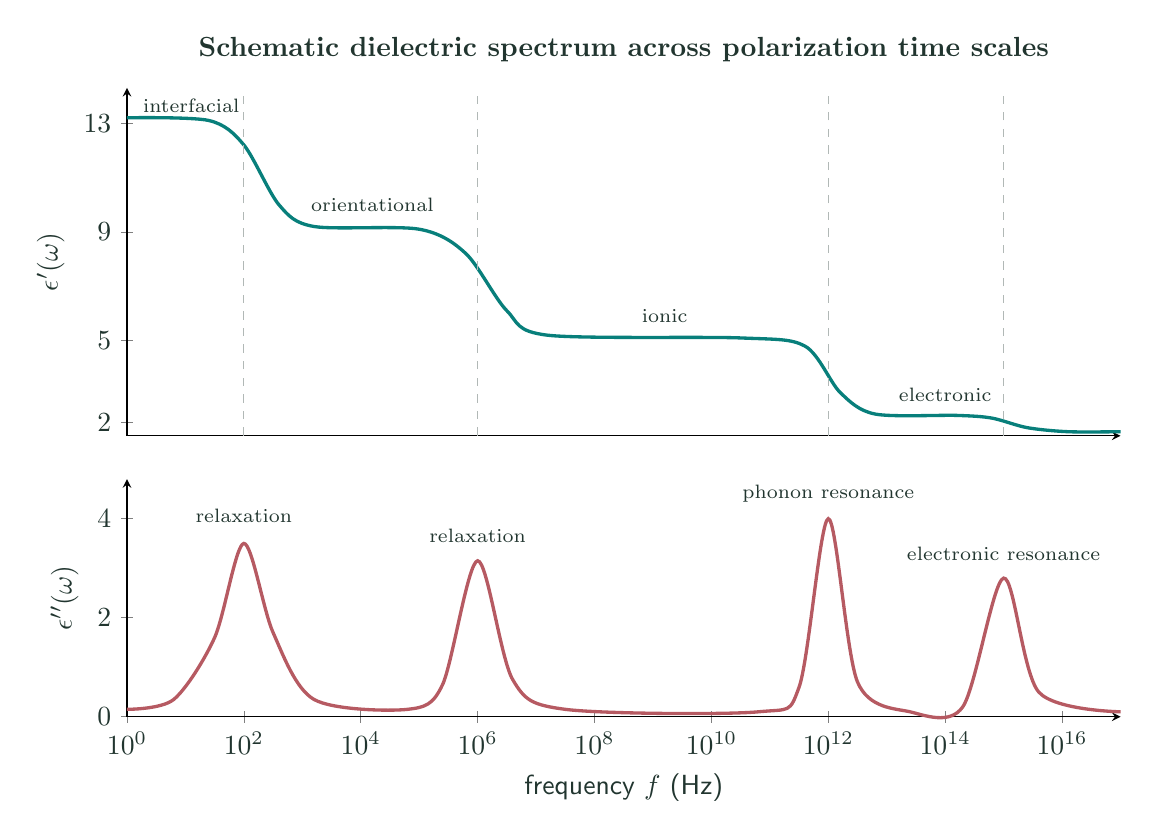
\begin{tikzpicture}[font=\sffamily,text=ink]
\begin{axis}[
  name=real,width=14.2cm,height=6.0cm,
  xmin=0,xmax=17,ymin=1.5,ymax=14.3,
  axis lines=left,xtick=\empty,ytick={2,5,9,13},
  ylabel={$\epsilon'(\omega)$},
  title={Schematic dielectric spectrum across polarization time scales},
  title style={font=\bfseries},
  every axis plot/.append style={very thick},
  clip=false]
  \addplot[teal,smooth] coordinates {(0,13.2)(1.4,13.1)(2.0,12.2)(2.6,10.0)(3.2,9.2)(5.0,9.1)(5.8,8.2)(6.5,6.1)(7.2,5.2)(10.5,5.1)(11.6,4.8)(12.2,3.1)(12.8,2.3)(14.2,2.25)(14.8,2.15)(15.4,1.8)(16.1,1.65)(17,1.65)};
  \draw[dashed,ink!35] (axis cs:2,1.5)--(axis cs:2,14.0);
  \draw[dashed,ink!35] (axis cs:6,1.5)--(axis cs:6,14.0);
  \draw[dashed,ink!35] (axis cs:12,1.5)--(axis cs:12,14.0);
  \draw[dashed,ink!35] (axis cs:15,1.5)--(axis cs:15,14.0);
  \node[font=\scriptsize,align=center] at (axis cs:1.1,13.65) {interfacial};
  \node[font=\scriptsize,align=center] at (axis cs:4.2,10.0) {orientational};
  \node[font=\scriptsize,align=center] at (axis cs:9.2,5.9) {ionic};
  \node[font=\scriptsize,align=center] at (axis cs:14.0,3.0) {electronic};
\end{axis}
\begin{axis}[
  at={(real.south west)},anchor=north west,yshift=-0.55cm,
  width=14.2cm,height=4.6cm,
  xmin=0,xmax=17,ymin=0,ymax=4.8,
  axis lines=left,xtick={0,2,4,6,8,10,12,14,16},
  xticklabels={$10^0$,$10^2$,$10^4$,$10^6$,$10^8$,$10^{10}$,$10^{12}$,$10^{14}$,$10^{16}$},
  xlabel={frequency $f$ (Hz)},ylabel={$\epsilon''(\omega)$},
  every axis plot/.append style={very thick},
  clip=false]
  \addplot[rose,smooth] coordinates {(0,0.15)(0.8,0.35)(1.5,1.6)(2.0,3.5)(2.5,1.7)(3.2,0.35)(4.8,0.15)(5.4,0.65)(6.0,3.15)(6.6,0.75)(7.5,0.15)(10.8,0.1)(11.5,0.6)(12.0,4.0)(12.5,0.7)(13.4,0.1)(14.3,0.2)(15.0,2.8)(15.6,0.5)(17,0.1)};
  \node[font=\scriptsize] at (axis cs:2.0,4.05) {relaxation};
  \node[font=\scriptsize] at (axis cs:6.0,3.65) {relaxation};
  \node[font=\scriptsize] at (axis cs:12.0,4.5) {phonon resonance};
  \node[font=\scriptsize] at (axis cs:15.0,3.3) {electronic resonance};
\end{axis}
\end{tikzpicture}
\end{document}
